% =============================================================================
%  The CLAS12 Simulation Portal to the Open Science Grid (simGrid)
%
%  Main file. The preamble (document class, packages, house style) is in
%  simgrid_osg_portal_preamble.tex. The body is one file per chapter under
%  chapters/, inputted through simgrid_osg_portal_doc.tex.
% =============================================================================

\input{simgrid_osg_portal_preamble}

\begin{document}

\pagestyle{fancy}
\fancyhf{}
\renewcommand{\headrulewidth}{0.4pt}
\renewcommand{\sectionmark}[1]{\markright{\thesection.\ #1}}
\fancyhead[L]{\footnotesize\slshape simGrid}
\fancyhead[R]{\footnotesize\slshape \rightmark}
\fancyfoot[L]{\small\slshape Jefferson Lab}
\fancyfoot[R]{\small\slshape M. Ungaro}
\fancyfoot[C]{\small\thepage}

% ============================ FRONT MATTER ===================================

\thispagestyle{plain}
\notetitle{The CLAS12 Simulation Portal to the\\ Open Science Grid (simGrid)}
\vspace{18pt}
\noteauthor{M. Ungaro}
\vspace{8pt}
\noteaffiliation{Jefferson Lab, 12,000 Jefferson Avenue, 23606 Newport News, VA, USA}
\vspace{6pt}

% ============================ ABSTRACT ===========================================

\begin{noteabstract}

The CLAS12 collaboration uses the Open Science Grid (OSG) to run Monte-Carlo simulations
for its various experiments.

The software framework that oversees the simulations workflow is \texttt{simGrid}.
It has two main components: a web portal runs on a dedicated server, collects and indexes
user requests in a dedicated MYSQL database; and a set of scripts on the HTCondor node that
submit the queue to the OSG\@.

Each worker node runs the full CLAS12 chain - generator, GEMC, background merging,
denoising, reconstruction, and DST creation --- and writes the
result back to Jefferson Lab volatile storage through the Pelican platform.

\texttt{simGrid} implements two fair-share mechanisms: a database-side queue that orders
requests across users, and algorithms to balance the running submissions.

\end{noteabstract}

% ============================ KEYWORDS ===========================================


\begin{center}
\begin{minipage}{0.86\textwidth}
\small\textbf{Keywords:} CLAS12, GEMC, Open Science Grid (OSG), HTCondor, Pelican, fair-share
scheduling, Monte-Carlo production.
\end{minipage}
\end{center}
\vspace{6pt}


% ---------------------------------------------------------------------------
% Table of Contents --- optional. Uncomment \tableofcontents below to enable it.
% Choose how much it lists with the tocdepth counter:
\setcounter{tocdepth}{1}  % chapters only (the top-level \section entries)
%   \setcounter{tocdepth}{2}  % also include their sections (the \subsection entries)
% ---------------------------------------------------------------------------
% \setcounter{tocdepth}{2}
\tableofcontents

% ============================ BODY ===========================================

% Body driver: one \input per chapter (chapters/), then the appendices.

\section{Overview}\label{ch:1}

CLAS12 analyses depend on large Monte-Carlo statitics produced with the same software, geometry, and fields
configuration as the reconstructed data.

Running simulations by hand, on the OSG or the JLab farm, involves writing the submision configuration files
that contain the generator, Monte-Carlo and reconstruction conditions, chaining the pipeline outputs,
and copying results back. Given the growing number of experiments, configurations, geometry, field, and software versions,
this is error-prone and not easily reproducible.

simGrid solves this: any authenticated collaborator can request a self-consistent Monte-Carlo workflow from a browser,
with the correct software versions, field maps, vertex handling, and background merging selected for them,
and have it run at scale on the OSG without touching HTCondor directly.
The portal is the single, reproducible path from a physics request to a DST.



\subsection{Design goals and constraints}

The system is shaped by three goals and one constraint:

\begin{itemize}
  \item \textbf{Self-service:} a user with no grid or software expertise can submit a correct workflow from a form.
  \item \textbf{Operability:} the submission pipeline is self-documenting and reproducible.
  \item \textbf{Fair sharing:} no single user can monopolize the shared allocation; waiting requests are
  ordered by a history-weighted, load-aware queue.
\end{itemize}

The constraint is that \textbf{all jobs run under one shared HTCondor owner, \texttt{gemc}.} OSG allocations
and OAuth credentials are granted to that single identity, not to individual collaborators. Fair sharing
therefore cannot be delegated to HTCondor's per-user accounting; the portal must implement it itself. This
constraint is the reason the two priority systems (Chapters 10 and 11) exist and are kept separate.



\subsection{Terminology and conventions}

\begin{itemize}
  \item \textbf{Submission / cluster / subjob / job.} A \textit{submission} is a single portal request.
  When submitted to OSG, it becomes a HTCondor \textit{cluster}. A cluster contains many \textit{subjobs}
  (HTCondor processes, \texttt{\$(Process)}). Here we will use subjob and job interchangeably: a submission
  can request to run 10,000 jobs; correspondigly, the created cluster will contain 10,000 subjobs.
  \item \textbf{scard} The \textit{scard} (steering card) is the key:value dictionary the portal produces
  from the user request and stores in the database; it drives all the downstream generation.
  \item \textbf{Type-1 vs. type-2.} A \textit{type-1} submission runs an event generator on the worker node to
  produce events; a \textit{type-2} submission consumes pre-generated LUND files from a
  \texttt{/\allowbreak{}volatile/\allowbreak{}clas12/\allowbreak{}} directory, one subjob per file. The type is
  inferred from the generator field (Chapter 4).
\end{itemize}

\section{The Web Portal (User-Facing Layer)}\label{ch:3}

\subsection{Page map and navigation}

The portal is a small set of PHP pages sharing a common header/footer (\texttt{header.\allowbreak{}php}, \texttt{head.\allowbreak{}php}): \texttt{index} (landing and links), \texttt{type1} (generator submission form), \texttt{type2} (LUND-file submission form), \texttt{monitor} (submissions table), \texttt{fairshare} (queue view), \texttt{osgStats} (OSG-level statistics), and \texttt{about} (documentation and generator-testing guidance). A maintenance variant (\texttt{indexMaintanance.\allowbreak{}php}) replaces the landing page during downtime.

\subsection{Environment/mode detection}

\texttt{common.\allowbreak{}php} centralizes environment detection so every page renders consistently in production or development. Development mode is recognized from the request URL and switches the database target, container tag, and operational banners. This keeps a single codebase serving both \texttt{CLAS12OCR}/production and \texttt{CLAS12TEST}/devel without per-page conditionals.

\subsection{Submission form: Generator jobs (type-1)}

\texttt{type1.\allowbreak{}php} presents the generator workflow (Figure --- portal screenshot to be added). Fields: configuration, software versions (\texttt{softwarev}), MC generator version (\texttt{mcgenv}), optional run selection, magnetic fields, vertex handling (z adjustment, beamspot smear, raster, generator-vertex mode), generator and its options, events per job (1--5000), number of jobs (0--10000), background merging, an optional string identifier, and output type (DST or GEMC-only). The event and job caps are enforced as HTML \texttt{min}/\texttt{max} attributes and re-checked in \texttt{main.\allowbreak{}js}.

\subsection{Submission form: LUND-file jobs (type-2)}

\texttt{type2.\allowbreak{}php} presents the pre-generated-input workflow. Instead of a generator, the user supplies a web location under \texttt{/\allowbreak{}volatile/\allowbreak{}clas12/\allowbreak{}} containing LUND files. The model is \textit{one subjob per file}: the number of jobs is determined by the number of files found, not entered by the user. All other configuration (fields, vertex, software, background merging, output type) mirrors type-1.

\subsection{Client-side logic (\texttt{main.\allowbreak{}js})}

\texttt{main.\allowbreak{}js} drives the dynamic form: it populates the configuration, software-version, and generator-version pickers; recomputes the total-events field from events-per-job $\times$ jobs; enforces the event/job caps; shows or hides the run-by-run UI; and formats the read-only vertex/beamspot/raster fields from the chosen configuration. It is the first line of input validation before anything is written server-side.

\subsection{From form to scard}

\texttt{submit\_\allowbreak{}type1.\allowbreak{}php} and \texttt{submit\_\allowbreak{}type2.\allowbreak{}php} receive the POST, sanitize the fields, and write the scard as key:value lines (Chapter 4). The scard is the only representation of the request that travels downstream; the PHP layer's job is to produce a correct, well-formed scard and hand it to the uploader.

\subsection{Invoking the uploader}

Each submit page then \texttt{exec}s \texttt{db\_\allowbreak{}io/\allowbreak{}upload\_\allowbreak{}submission.\allowbreak{}py} with the scard, writing a per-submission log file so that a failed upload can be diagnosed from the web tier. The uploader performs the database insert and the queue renumbering; the PHP page reports success or the captured error to the user.

\subsection{Job summary, details modal, and progress display}

After submission the portal shows a job summary. \texttt{get\_\allowbreak{}submission\_\allowbreak{}details.\allowbreak{}php} renders a details modal for a single submission --- its scard (aligned key:value lines), submission and processing timestamps, status, and priority. The \texttt{monitor} page renders the full table and a progress/estimated-time column derived from the monitoring snapshots (Chapter 13).

\subsection{Authentication and identity}

The portal identifies the user from the web-server-provided \texttt{REMOTE\_\allowbreak{}USER} and records \texttt{REMOTE\_\allowbreak{}ADDR}. The username determines the per-user output namespace on OSDF (\texttt{.\allowbreak{}.\allowbreak{}.\allowbreak{}/\allowbreak{}osg/\allowbreak{}<user>/\allowbreak{}<sub\_\allowbreak{}id>/\allowbreak{}}) and the user attribution used by the fair-share calculation. There is one shared grid identity (\texttt{gemc}) but many portal identities.

\subsection{Maintenance mode and operational banners}

During maintenance the landing page is swapped for \texttt{indexMaintanance.\allowbreak{}php}, and \texttt{common.\allowbreak{}php} banners signal development mode. These operational affordances prevent submissions during known-bad windows and make the active environment unambiguous to the user.

\subsection{Input handling and security considerations}

Because the PHP tier eventually hands strings to a shell (\texttt{exec} of the uploader) and to the scard parser, input handling matters: fields are escaped, shell arguments are quoted (\texttt{escapeshellarg}), and the string identifier is restricted at the input to an alphanumeric/hyphen character class. Filenames and paths are sanitized before use. Chapter 16 treats the trust model in full.

\section{The Steering Card (scard) and Configuration Model}\label{ch:4}

\subsection{Scard format and provenance}

The scard is a plain-text list of \texttt{key:\allowbreak{} value} lines produced by the portal and stored verbatim in the \texttt{submissions.\allowbreak{}scard} column. It is the single, human-readable contract between the web tier and the submission engine; every generation step reads from it and nothing else.

\subsection{The \texttt{SConfiguration} class}

\texttt{SConfiguration} (in \texttt{SConfiguration.\allowbreak{}py}) parses the scard into typed attributes. It can be built from a file (\texttt{SConfiguration(path)}) or from a string fetched from the database (\texttt{SConfiguration.\allowbreak{}from\_\allowbreak{}string}). Parsing is forward-compatible: a \texttt{key:\allowbreak{} value} whose key matches a known attribute sets that attribute; any unknown key is preserved in an \texttt{\_\allowbreak{}extra} dictionary rather than raising, so new scard fields do not break older engine versions. The literal key \texttt{file} is ignored.

\subsection{Submission-type resolution}

If the scard does not state a type, \texttt{\_\allowbreak{}resolve\_\allowbreak{}type()} infers it from the generator field: a value that starts with \texttt{/\allowbreak{}} or contains \texttt{:\allowbreak{}/\allowbreak{}/\allowbreak{}} is a path or URL to LUND files and yields \textbf{type 2}; anything else is a generator name and yields \textbf{type 1}. An explicit type in the scard is never overridden.

\subsection{Software-version resolution}

\texttt{\_\allowbreak{}resolve\_\allowbreak{}software\_\allowbreak{}versions()} unpacks the \texttt{softwarev} field --- a space-separated list of \texttt{name/\allowbreak{}version} tokens --- into \texttt{gemcv}, \texttt{coatjavav}, and \texttt{mcgenv} for \texttt{gemc}, \texttt{coatjava}, and \texttt{mcgen} respectively. It also derives \texttt{torus} and \texttt{solenoid} scale factors from a \texttt{fields} value of the form \texttt{tor<T>\_\allowbreak{}sol<S>} when they are not given directly. This lets the portal store one compact \texttt{fields} string while the engine sees explicit torus and solenoid values.

\subsection{Field reference}

The complete scard field reference --- every key, its meaning, default, and the components that consume it --- is given in Appendix A. The most consequential fields are \texttt{type}, \texttt{generator}, \texttt{configuration}, \texttt{softwarev}, \texttt{fields}, \texttt{nevents}/\texttt{njobs} (type-1), \texttt{bkmerging}, \texttt{output\_\allowbreak{}type}, \texttt{string\_\allowbreak{}id}, \texttt{vertex\_\allowbreak{}choice}/\texttt{zposition}/ \texttt{raster}, and the run-by-run \texttt{runs}/\texttt{run\_\allowbreak{}list}.

\subsection{Output-type semantics}

\texttt{output\_\allowbreak{}type =\allowbreak{} 1} selects the GEMC-only pipeline: the worker node runs the generator (or fetches LUND) and GEMC, optionally merges background, then uploads the GEMC output directly, skipping denoising, reconstruction, and DST creation. The default (\texttt{output\_\allowbreak{}type =\allowbreak{} 0}) runs the full chain to a DST. This single flag branches both the worker-node generator (Chapter 9) and the file chain.

\section{Data Model and Database Layer}\label{ch:5}

\subsection{The \texttt{submissions} table}

\texttt{submissions} is the central table. Each row is one portal request keyed by \texttt{user\_\allowbreak{}submission\_\allowbreak{}id}. Its lifecycle fields are \texttt{run\_\allowbreak{}status} (Chapter 6), \texttt{client\_\allowbreak{}time} (upload time), \texttt{server\_\allowbreak{}time} (set when the engine serves the row), \texttt{pool\_\allowbreak{}node} (the HTCondor \texttt{ClusterId} once submitted), and \texttt{priority} (the pending queue position). The request itself is the \texttt{scard}; the generated artifacts \texttt{runscript\_\allowbreak{}text} and \texttt{clas12\_\allowbreak{}condor\_\allowbreak{}text} are stored back for reproducibility. The full DDL is in Appendix B.

\subsection{The \texttt{users} table and provisioning}

\texttt{ensure\_\allowbreak{}user()} guarantees a \texttt{users} row exists for a portal username before a submission is inserted, creating it on first use. This keeps user attribution --- used by the fair-share calculation and the output namespace --- consistent without a separate registration step.

\subsection{Snapshot tables}

\texttt{owner\_\allowbreak{}submission\_\allowbreak{}snapshots} stores periodic JSON snapshots of the joined submissions view (Chapter 13), each with a \texttt{snapshot\_\allowbreak{}id} and \texttt{update\_\allowbreak{}time}. Fair-share views are similarly snapshotted. Snapshots decouple the portal display from live HTCondor queries and provide the history used for progress and completion detection.

\subsection{The \texttt{Database} wrapper}

\texttt{db\_\allowbreak{}io/\allowbreak{}database.\allowbreak{}py} wraps all database access: connection and credential handling (credentials read from a connection file such as \texttt{msql\_\allowbreak{}conn.\allowbreak{}txt}), \texttt{query\_\allowbreak{}one}/query helpers, the insert and renumber operations, the advisory-lock context manager, and the snapshot read/write/prune operations. Callers never issue raw connection management; they use these helpers.

\subsection{Stored generated artifacts}

After the engine generates the worker-node and HTCondor scripts, it persists them to the row (\texttt{runscript\_\allowbreak{}text}, \texttt{clas12\_\allowbreak{}condor\_\allowbreak{}text}). This makes each submission self-describing: the exact scripts that ran can be recovered from the database and compared (the container-parity checks of Chapter 15 rely on this).

\subsection{Concurrency control: the pending-priority advisory lock}

All operations that read-modify-write the pending queue are serialized with a MySQL advisory lock (\texttt{GET\_\allowbreak{}LOCK}/\texttt{RELEASE\_\allowbreak{}LOCK}, name \texttt{simgrid\_\allowbreak{}pending\_\allowbreak{}priorities}), exposed as the \texttt{pending\_\allowbreak{}priority\_\allowbreak{}lock} context manager. This prevents two concurrent inserts or status transitions from producing duplicate or gapped priorities.

\subsection{The contiguous \texttt{1.\allowbreak{}.\allowbreak{}N} invariant}

Only \texttt{Not Submitted} rows carry a positive priority, and those priorities always form a contiguous \texttt{1.\allowbreak{}.\allowbreak{}N} sequence with 1 next to run. \texttt{build\_\allowbreak{}contiguous\_\allowbreak{}priority\_\allowbreak{}updates()} re-derives this sequence from the current queue order --- preserving existing order, placing legacy priority-0 rows at the tail --- and every insert or status transition re-compacts to \texttt{1.\allowbreak{}.\allowbreak{}N} under the lock. The invariant is what lets the engine simply ask for "priority 1" and lets the fair-share calculator overwrite positions wholesale.

\section{Submission State Machine}\label{ch:6}

\subsection{Status vocabulary}

Statuses are defined once in \texttt{statuses.\allowbreak{}py} and never written as bare strings: \texttt{Not
Submitted}, \texttt{Processing}, \texttt{Submitted to OSG}, \texttt{Completed}, \texttt{Submission scripts
generated}, and the terminal \texttt{Failed to Read Directory}. Comparisons import these constants.

\subsection{State-transition diagram}

\begin{figure}[htbp]
  \centering
  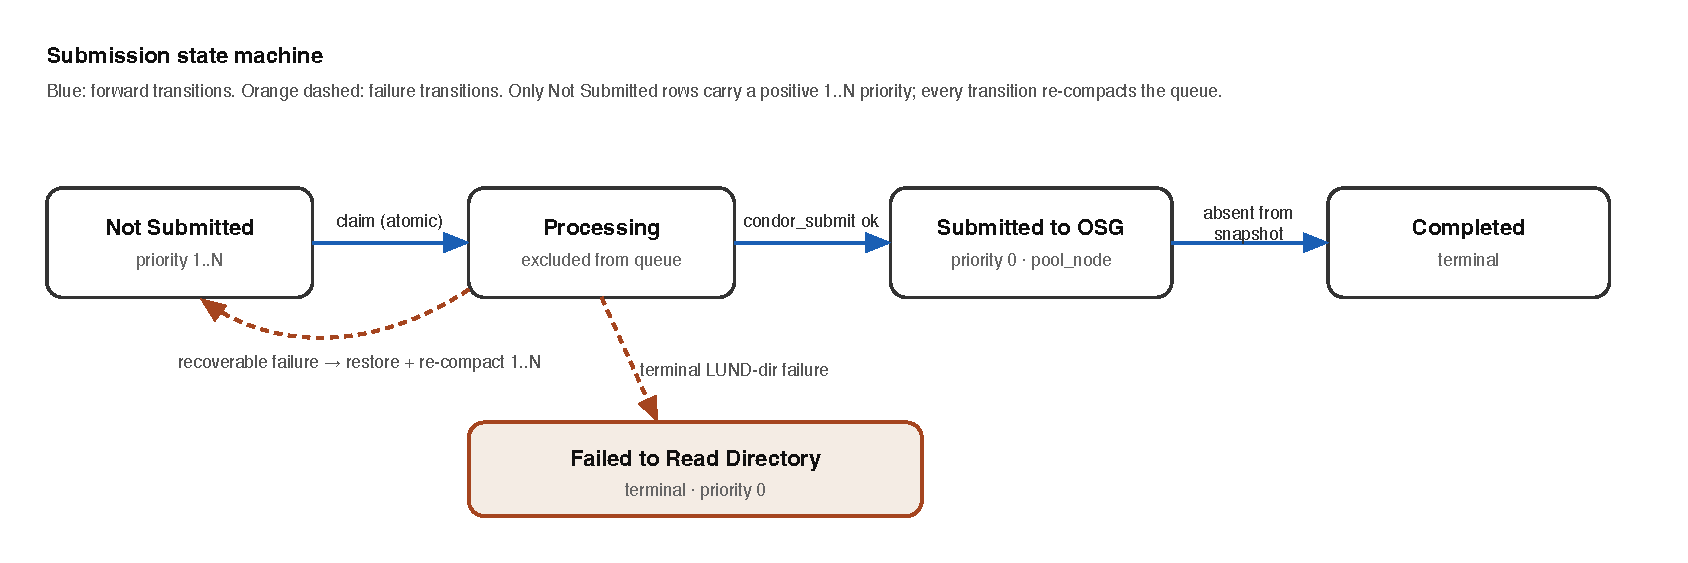
\includegraphics[width=\textwidth]{figures/fig2_state_machine}
  \caption{Submission state machine. States are defined once in \texttt{statuses.py}; the claim (Not Submitted
  $\rightarrow$ Processing) is an atomic status change, so at most one engine invocation submits a row. Only
  Not Submitted rows carry a positive $1..N$ priority, and every transition re-compacts the queue.}
  \label{fig:statemachine}
\end{figure}

\subsection{Priority values per state}

\texttt{Not Submitted} rows hold a unique pending position \texttt{1.\allowbreak{}.\allowbreak{}N}.
\texttt{Processing} rows are excluded from the pending queue. \texttt{Submitted to OSG} and \texttt{Failed to
Read Directory} rows hold priority \texttt{0} (they are out of the queue). The mapping is summarized in the
transitions table of Chapter 6.7 and the README.

\subsection{Atomic claim and race avoidance}

\texttt{mark\_\allowbreak{}submission\_\allowbreak{}processing()} performs the claim as an atomic status change
from \texttt{Not Submitted} to \texttt{Processing}. If another engine invocation claimed the row first, the
update affects no rows and the caller exits without submitting. This is what makes it safe to run the engine
concurrently or with an explicit \texttt{-\allowbreak{}b ID} target.

\subsection{Terminal and recoverable failure handling}

If \texttt{condor\_\allowbreak{}submit} is not reached, the row is restored to \texttt{Not Submitted} and the
queue re-compacted --- the request simply returns to the pending queue. A type-2 submission whose LUND
directory cannot be read is a terminal failure: the row receives \texttt{Failed to Read Directory} and priority
0, and is not retried.

\subsection{Invariants and idempotency}

Two invariants hold across all transitions: the pending queue is always contiguous
\texttt{1.\allowbreak{}.\allowbreak{}N}, and a row can be claimed by at most one engine invocation. Together
they make the engine idempotent --- re-running it never double-submits a request and never corrupts the queue.

\section{Job Submission Mechanism (\texttt{osg\_\allowbreak{}submit.\allowbreak{}py})}\label{ch:7}

\subsection{Invocation model}

\texttt{osg\_\allowbreak{}submit.\allowbreak{}py} is the submission engine, run from a cron wrapper on the submit node (one invocation processes one submission) or manually. Flags: \texttt{-\allowbreak{}-\allowbreak{}test} (skip the capacity check, mock Pelican), \texttt{-\allowbreak{}-\allowbreak{}devel} (use \texttt{CLAS12TEST} and the devel image), \texttt{-\allowbreak{}b ID} (target a specific submission), \texttt{-\allowbreak{}-\allowbreak{}target-\allowbreak{}site SITE} (pin all subjobs to one OSG site), and the \texttt{-\allowbreak{}-\allowbreak{}print-\allowbreak{}*} inspection flags.

\subsection{Step 1 --- capacity / back-pressure check}

The engine queries HTCondor for the running + idle jobs owned by \texttt{gemc}. If that exceeds \texttt{-\allowbreak{}-\allowbreak{}max-\allowbreak{}submitted-\allowbreak{}jobs} (default 80,000), the invocation exits without submitting. Back-pressure is a normal outcome, not an error: it simply defers work until the pool drains. \texttt{-\allowbreak{}-\allowbreak{}test} skips this check.

\subsection{Step 2 --- fetching the next job}

\texttt{return\_\allowbreak{}unsubmitted\_\allowbreak{}job()} selects the \texttt{Not Submitted} row with the smallest \textit{positive} priority; legacy priority-0 rows are treated as the tail of the queue rather than being ignored. With \texttt{-\allowbreak{}b ID} the engine targets that submission explicitly instead of choosing priority 1.

\subsection{Step 3 --- parsing the scard and claiming the row}

The \texttt{scard} is parsed into an \texttt{SConfiguration}, and the row is atomically claimed (\texttt{Not Submitted} $\rightarrow$ \texttt{Processing}, Chapter 6.4), after which the remaining pending priorities are compacted to \texttt{1.\allowbreak{}.\allowbreak{}N}.

\subsection{Step 3b --- staging-directory layout}

A per-submission staging directory is created:

\begin{lstlisting}
~/osgOutput/<username>/job_<user_submission_id>/
    log/     <- HTCondor per-subjob .out / .err / .log
\end{lstlisting}

The generated \texttt{clas12.\allowbreak{}condor}, \texttt{nodescript.\allowbreak{}sh}, \texttt{functions.\allowbreak{}sh}, and (type-2) \texttt{lund\_\allowbreak{}files} are written here.

\subsection{Step 4 --- type-2 LUND enumeration and validation}

For type-2, the generator field must start with \texttt{/\allowbreak{}volatile/\allowbreak{}clas12/\allowbreak{}} --- enforced before any file operation. \texttt{pelican object ls} enumerates the LUND files (\texttt{.\allowbreak{}dat}, \texttt{.\allowbreak{}txt}, \texttt{.\allowbreak{}lund}) on the OSDF mirror; each URI is written as one line to \texttt{lund\_\allowbreak{}files}, and HTCondor creates one subjob per line. In \texttt{-\allowbreak{}-\allowbreak{}test} mode a three-file mock is used when Pelican is unavailable.

\subsection{Step 4b --- run-by-run staging}

For run-dependent requests, the run set (\texttt{runs.\allowbreak{}json} / \texttt{run\_\allowbreak{}list.\allowbreak{}txt}) is staged so the worker node can draw a weighted run per subjob (\texttt{select\_\allowbreak{}run.\allowbreak{}py}, Chapter 9.6.2). This spans both submission staging and runtime selection.

\subsection{Step 5 --- generating the HTCondor submit file}

\texttt{generate\_\allowbreak{}condor\_\allowbreak{}card()} assembles \texttt{clas12.\allowbreak{}condor} from nine section generators in fixed order (Chapter 8).

\subsection{Step 6 --- generating the nodescript and staging scripts}

\texttt{generate\_\allowbreak{}nodescript()} assembles \texttt{nodescript.\allowbreak{}sh}; it and \texttt{functions.\allowbreak{}sh} are staged into the directory, and both generated texts are persisted to the database (Chapter 5.5).

\subsection{Step 7 --- \texttt{condor\_\allowbreak{}submit} and finalization}

The engine runs \texttt{condor\_\allowbreak{}submit} in the staging directory, captures the returned \texttt{ClusterId}, and on success sets \texttt{run\_\allowbreak{}status =\allowbreak{} 'Submitted to OSG'}, records \texttt{server\_\allowbreak{}time} and \texttt{pool\_\allowbreak{}node =\allowbreak{} ClusterId}, clears the pending priority, and re-compacts the queue.

\subsection{Failure / rollback semantics}

A \texttt{finally} path restores a not-yet-submitted row to \texttt{Not Submitted} and re-compacts the queue, so a crash between claim and submit cannot strand a request in \texttt{Processing}. Terminal LUND failures instead set \texttt{Failed to Read Directory} (Chapter 6.5). Error artifacts are left in the staging directory for diagnosis.

\subsection{Test-mode behavior and DB-write guards}

\texttt{-\allowbreak{}-\allowbreak{}test} performs no MySQL status update and does not invoke \texttt{condor\_\allowbreak{}submit}; combined with \texttt{-\allowbreak{}-\allowbreak{}print-\allowbreak{}*} it is the standard way to inspect a generated card or nodescript for any submission without side effects.

\section{HTCondor Submit-File Generation (\texttt{generators/\allowbreak{}condor/\allowbreak{}})}\label{ch:8}

\subsection{Assembly model}

\texttt{generate\_\allowbreak{}condor\_\allowbreak{}card()} calls one generator per section and joins their
strings in a fixed order: header, retry policy, requirements, undesired sites, authentication, hardware,
executable, file transfer, and queue (always last). Each generator is a pure function of the scard plus
optional overrides, so a submission's card is fully determined by its scard and the call parameters. Adding a
section means adding a function and one line to the assembly list.

\subsection{Header}

\texttt{create\_\allowbreak{}header()} sets \texttt{Universe =\allowbreak{} vanilla} (the only universe
supported for OSG pilots), the CVMFS-hosted Singularity image (\texttt{clas12software:\allowbreak{}production},
or \texttt{:\allowbreak{}devel} when \texttt{devel=\allowbreak{}True}), \texttt{+SingularityBindCVMFS
=\allowbreak{} True} to expose all of \texttt{/\allowbreak{}cvmfs} inside the container, and a \texttt{Rank}
expression built from a site-preference table (\texttt{SITE\_\allowbreak{}RANKS}; e.g. Glasgow 300, CNAF 200,
default 100, Syracuse deprioritized).

\subsection{Retry / hold policy}

\texttt{create\_\allowbreak{}retry\_\allowbreak{}policy()} encodes eviction tolerance:
\texttt{on\_\allowbreak{}exit\_\allowbreak{}remove} removes only clean exits (no signal, code 0);
\texttt{on\_\allowbreak{}exit\_\allowbreak{}hold} holds any signalled or non-zero exit;
\texttt{periodic\_\allowbreak{}release} releases a held job back to idle only when it has been retried fewer
than 5 times, has been held over an hour, and exited with one of the known transient OSG codes (202, 204--208,
210--213 --- CVMFS unavailable, pilot evicted, etc.). Anything else stays held for inspection. The exit-code
taxonomy is in Appendix E.

\subsection{Requirements}

\texttt{create\_\allowbreak{}requirements()} guards against known infrastructure failures:
\texttt{HAS\_\allowbreak{}SINGULARITY}, the OSG oasis CVMFS repository mounted, kernel $\geq$ 2.17, a
sufficiently recent CVMFS oasis revision, and glidein version $\geq$ 534.
\texttt{-\allowbreak{}-\allowbreak{}target-\allowbreak{}site} appends a \texttt{GLIDEIN\_\allowbreak{}Site
=\allowbreak{}=\allowbreak{} "<SITE>"} clause to pin all subjobs to one site.

\subsection{Undesired sites}

\texttt{create\_\allowbreak{}undesired()} emits a \texttt{+UNDESIRED\_\allowbreak{}Sites} exclusion list,
keeping jobs off sites known to fail for CLAS12 workloads.

\subsection{Authentication}

\texttt{create\_\allowbreak{}authentication()} emits \texttt{use\_\allowbreak{}oauth\_\allowbreak{}services
=\allowbreak{} jlab\_\allowbreak{}clas12}. The submit node's CredMon obtains an OAuth2 bearer token for that
service; HTCondor injects it as \texttt{BEARER\_\allowbreak{}TOKEN\_\allowbreak{}FILE} into the job
environment, where Pelican/OSDF use it to read LUND input and write HIPO output. No long-lived secret ever
reaches the node.

\subsection{Hardware}

\texttt{create\_\allowbreak{}hardware()} requests the GEMC resource profile: 1 CPU (GEMC is single-threaded),
2.256 GB memory (GEMC peak RSS $\approx$ 1.8 GB plus headroom), and 2 GB scratch disk. Overrides exist for
heavier workloads.

\subsection{Executable}

\texttt{create\_\allowbreak{}executable()} names \texttt{nodescript.\allowbreak{}sh} as the executable, sets
the per-subjob \texttt{log}/\texttt{out}/\texttt{err} paths under \texttt{log/\allowbreak{}}, and sets
\texttt{+ProjectName} for OSG accounting.

\subsection{File transfer}

\texttt{create\_\allowbreak{}file\_\allowbreak{}transfer()} stages \texttt{nodescript.\allowbreak{}sh} and
\texttt{functions.\allowbreak{}sh} in (\texttt{should\_\allowbreak{}transfer\_\allowbreak{}files =\allowbreak{}
YES}, \texttt{when\_\allowbreak{}to\_\allowbreak{}transfer\_\allowbreak{}output =\allowbreak{}
ON\_\allowbreak{}EXIT}) and retrieves only the \texttt{output/\allowbreak{}} subdirectory. Notably, type-2 LUND
files are \textbf{not} staged through HTCondor: the worker node fetches each file on-node via Pelican, avoiding
saturation of the submit node with large LUND directories.

\subsection{Queue}

\texttt{create\_\allowbreak{}queue()} is the final section. Type-1 emits \texttt{Arguments =\allowbreak{}
\$(Process)} and \texttt{Queue N} (N = \texttt{njobs}). Type-2 uses itemdata: \texttt{Arguments =\allowbreak{}
\$(Process) \$(lundFile)} and \texttt{queue lundFile from lund\_\allowbreak{}files}, expanding the staged
\texttt{lund\_\allowbreak{}files} one line per subjob.

\subsection{Extending the card}

Because each section is an independent pure function joined in order, a new section (say, a new accounting
attribute or a new requirement) is added by writing one generator and inserting one call in
\texttt{generate\_\allowbreak{}condor\_\allowbreak{}card()} --- no template surgery. An annotated full card is
in Appendix C.

\section{Worker-Node Execution Pipeline (\texttt{nodescript.\allowbreak{}sh} / \texttt{functions.\allowbreak{}sh})}\label{ch:9}

\subsection{Self-documenting nodescript convention}

Every pipeline step in the generated \texttt{nodescript.\allowbreak{}sh} follows the same four-part pattern: a \texttt{\# input:\allowbreak{} \ldots{} output:\allowbreak{} \ldots{}} comment, an explicit \texttt{cmd=\allowbreak{}(.\allowbreak{}.\allowbreak{}.\allowbreak{})} bash array holding the full invocation, a descriptive \texttt{echo "Running <Step>:\allowbreak{} \$\{cmd[@]\}"}, and \texttt{run\_\allowbreak{}timed <fn> "\$\{cmd[@]\}"} which times the step and forwards the command to a thin wrapper in \texttt{functions.\allowbreak{}sh}. The wrappers add error handling and cleanup (removing intermediate files, \texttt{df} checks) but construct no commands. The result is a script a user can read top-to-bottom and re-run verbatim.

\subsection{Preamble}

\texttt{create\_\allowbreak{}preamble.\allowbreak{}py} emits the shebang, argument parsing (\texttt{sjob} = \texttt{\$1}; for type-2, \texttt{lundFile} = \texttt{\$2} and \texttt{lund\_\allowbreak{}base} derived from it), \texttt{set -\allowbreak{}euo pipefail}, the output directory, sourcing of \texttt{functions.\allowbreak{}sh}, and the exit-code definitions.

\subsection{Environment setup}

The script sets \texttt{CLAS12\_\allowbreak{}CONFIG} (the coatjava/gemc config tree on CVMFS), \texttt{OSRELEASE=\allowbreak{}almalinux9-\allowbreak{}gcc11} so CVMFS modulefiles resolve to the platform directory containing GEMC/JDK/HIPO/denoise, the module system, and \texttt{RCDB\_\allowbreak{}CONNECTION} for run conditions.

\subsection{Module-loading strategy}

Modules are loaded and unloaded per step with pinned versions (\texttt{gemc}, \texttt{coatjava}, \texttt{mcgen} from the scard), with availability checks, so each stage runs against exactly the requested software.

\subsection{Pelican / OSDF environment}

\texttt{BEARER\_\allowbreak{}TOKEN\_\allowbreak{}FILE} (injected by the CredMon via the Condor OAuth service) authorizes all Pelican transfers on the node --- LUND fetch and output upload alike.

\subsection{Input stage}

\texttt{create\_\allowbreak{}lund\_\allowbreak{}or\_\allowbreak{}generator.\allowbreak{}py} emits one of three input paths: \textbf{type-2} fetches the assigned LUND file with \texttt{pelican object get}; an \textbf{external generator} runs the generator command array to produce events; a \textbf{GEMC-internal generator} produces events inside GEMC and needs no separate input step.

\begin{itemize}
  \item \textbf{9.6.1 Seed generation.} External generators receive a per-subjob random seed so subjobs are statistically independent.
  \item \textbf{9.6.2 Run-by-run weighted selection.} For run-dependent requests, \texttt{select\_\allowbreak{}weighted\_\allowbreak{}run} (calling \texttt{select\_\allowbreak{}run.\allowbreak{}py}) draws a run number from the staged run list weighted by luminosity/exposure, so the sample reproduces the run-mix of real data. This is the runtime half of the run-by-run feature staged in Chapter 7.7.
\end{itemize}

\subsection{GEMC execution}

\texttt{create\_\allowbreak{}run\_\allowbreak{}gemc.\allowbreak{}py} resolves the gcard for the configuration and builds the full \texttt{cmd=\allowbreak{}(gemc \ldots{})} array: the gcard, number of events, torus/solenoid scales from \texttt{fields}, vertex/z-position and raster handling, beam settings, and the output \texttt{gemc.\allowbreak{}hipo}.

\subsection{Background merging}

When \texttt{bkmerging} is set, \texttt{fetch\_\allowbreak{}background\_\allowbreak{}file} pulls a random background HIPO file from OSDF and \texttt{merge\_\allowbreak{}background} merges it into the GEMC output over the configured detector list, producing \texttt{gemc.\allowbreak{}merged.\allowbreak{}hipo} (and removing the inputs).

\subsection{Denoising}

For coatjava older than 14, \texttt{run\_\allowbreak{}denoiser} (\texttt{denoise2.\allowbreak{}exe}) runs on the merged/GEMC file. For coatjava 14 and newer the step is skipped and reconstruction reads the merged (or plain) GEMC file directly.

\subsection{Reconstruction}

\texttt{run\_\allowbreak{}reconstruction} runs \texttt{recon-\allowbreak{}util} with the YAML appropriate to the request (an \texttt{mc-\allowbreak{}ai} configuration for AI-assisted tracking, or the experiment configuration), producing \texttt{recon.\allowbreak{}hipo}.

\subsection{Integrity test}

\texttt{test\_\allowbreak{}hipo\_\allowbreak{}file} runs \texttt{hipo-\allowbreak{}utils -\allowbreak{}test} on the reconstructed file to catch truncated or corrupt output before it is promoted to a DST.

\subsection{DST creation vs. rename}

\texttt{create\_\allowbreak{}dst} reduces the reconstructed file to the DST bank list, honoring \texttt{dstOUT}, producing the final \texttt{\$OUTPUT\_\allowbreak{}FILE}. In the GEMC-only branch there is no DST step --- the GEMC output is renamed to \texttt{\$OUTPUT\_\allowbreak{}FILE}.

\subsection{Output filename convention}

\texttt{get\_\allowbreak{}output\_\allowbreak{}filename} builds \texttt{\$OUTPUT\_\allowbreak{}FILE} as \texttt{<string\_\allowbreak{}id>-\allowbreak{}<submission\_\allowbreak{}id>-\allowbreak{}<sjob>.\allowbreak{}hipo} (type-1) or \texttt{<string\_\allowbreak{}id>-\allowbreak{}<lund\_\allowbreak{}base>-\allowbreak{}<submission\_\allowbreak{}id>-\allowbreak{}<sjob>.\allowbreak{}hipo} (type-2), so every subjob's output is uniquely named and traceable back to its submission.

\subsection{Output upload}

\texttt{write\_\allowbreak{}to\_\allowbreak{}jlab} uploads \texttt{\$OUTPUT\_\allowbreak{}FILE} to the per-user OSDF volatile namespace (\texttt{osdf:\allowbreak{}/\allowbreak{}/\allowbreak{}/\allowbreak{}jlab-\allowbreak{}osdf/\allowbreak{}clas12/\allowbreak{}volatile/\allowbreak{}osg/\allowbreak{}<user>/\allowbreak{}<sub\_\allowbreak{}id>/\allowbreak{}}).

\subsection{GEMC-only branch}

For \texttt{output\_\allowbreak{}type =\allowbreak{} 1}, the pipeline stops after GEMC (and optional background merging): the GEMC file is renamed to \texttt{\$OUTPUT\_\allowbreak{}FILE} and uploaded directly, skipping denoising, reconstruction, integrity test, and DST.

\subsection{Timing instrumentation}

\texttt{run\_\allowbreak{}timed} records each step's wall time in a timing registry, and \texttt{print\_\allowbreak{}timing\_\allowbreak{}summary} emits a per-step breakdown at the end of the job --- the basis for the timing figures and for spotting a slow stage.

\subsection{Exit-code taxonomy}

Each step maps failures to specific exit codes; the transient subset (Chapter 8.3) is exactly the set \texttt{periodic\_\allowbreak{}release} retries. This coupling --- the nodescript's exit codes and the Condor card's release policy --- is what turns transient OSG failures into automatic retries and real bugs into held jobs. The full catalogue is in Appendix E.

\subsection{The complete file chain}

\begin{figure}[htbp]
  \centering
  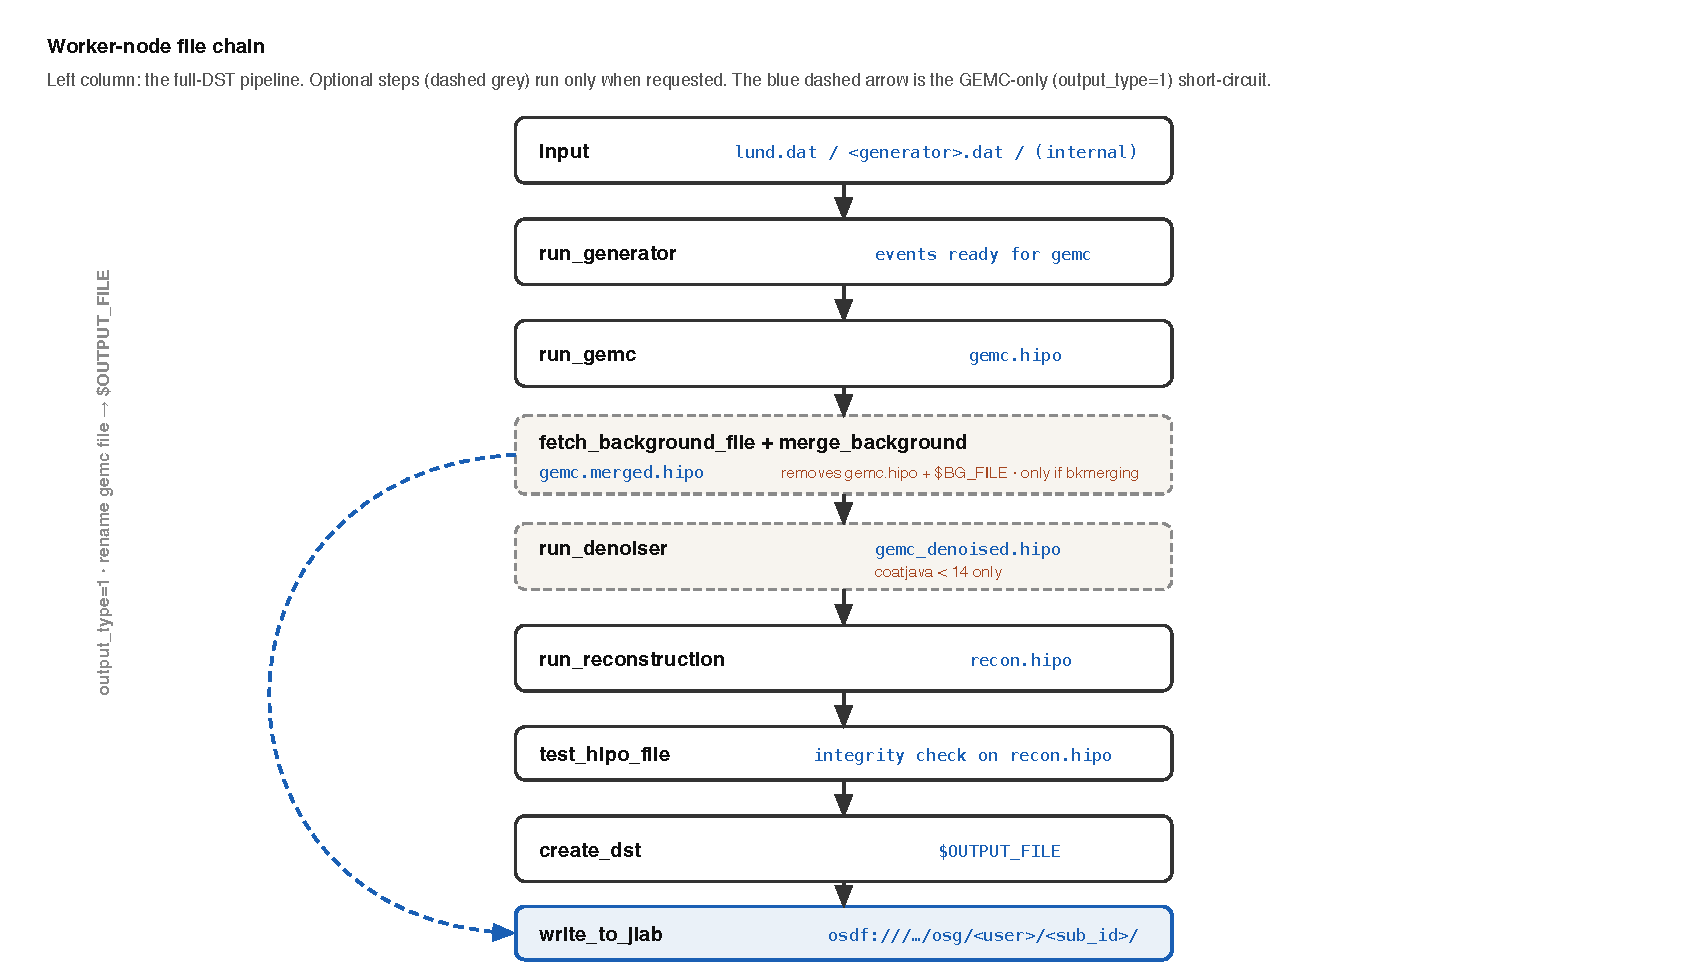
\includegraphics[width=0.8\textwidth]{figures/fig3_file_chain}
  \caption{Worker-node file chain. Left column: the full-DST pipeline. Optional steps run only when requested; the dashed arrow is the GEMC-only (\texttt{output\_type=1}) short-circuit that renames the GEMC output and uploads it directly.}
  \label{fig:filechain}
\end{figure}

\section{Pending-Submission Priority (Fair-Share Queue)}\label{ch:10}

\subsection{Problem statement}

Waiting requests (\texttt{Not Submitted}) from many portal users share one HTCondor owner. Something must
decide which waiting request the engine submits next. That is the job of the pending-submission priority,
computed by \texttt{db\_\allowbreak{}io/\allowbreak{}priority\_\allowbreak{}submissions.\allowbreak{}py}.

\subsection{Scope boundary}

\textbf{This system writes only \texttt{submissions.\allowbreak{}priority}. It never writes HTCondor
\texttt{JobPrio}.} It orders requests \textit{before} they are submitted; once a request is submitted it leaves
this queue entirely.

\subsection{Inputs}

The calculator reads the submission users, IDs, timestamps (\texttt{client\_\allowbreak{}time},
\texttt{server\_\allowbreak{}time}), and statuses from MySQL, and queries live HTCondor for the running-job
counts per user (mapping \texttt{ClusterId} $\rightarrow$ user through \texttt{pool\_\allowbreak{}node}).
Current occupancy is thus an input, but the output goes only to the MySQL queue.

\subsection{History-weighted load model}

Each user's load in the scoring denominator is \texttt{history\_\allowbreak{}load\_\allowbreak{}submitted +
history\_\allowbreak{}load\_\allowbreak{}pending}:

\begin{itemize}
  \item \textbf{10.4.1 Decayed submitted history.} Each non-pending job contributes
  \texttt{2\textasciicircum{}(-\allowbreak{}age/\allowbreak{}T\_\allowbreak{}h)}, where age is measured from
  \texttt{server\_\allowbreak{}time} (when the portal served it; \texttt{client\_\allowbreak{}time} as
  fallback) and \texttt{T\_\allowbreak{}h} is
  \texttt{-\allowbreak{}-\allowbreak{}history-\allowbreak{}half-\allowbreak{}life-\allowbreak{}days}. A job
  served now weighs 1; one served \texttt{T\_\allowbreak{}h} days ago weighs 0.5. Missing timestamps are
  treated as brand-new (weight 1), conservatively.
  \item \textbf{10.4.2 Raw pending load.} Each \texttt{Not Submitted} job contributes exactly 1, undecayed ---
  a queue penalty for having many requests waiting.
  \texttt{-\allowbreak{}-\allowbreak{}no-\allowbreak{}queue-\allowbreak{}penalty} forces this term to zero.
  \item \textbf{10.4.3 Combined load and exponent.} The two terms sum to the per-user load, and
  \texttt{-\allowbreak{}-\allowbreak{}queue-\allowbreak{}penalty-\allowbreak{}exponent} raises it to a power in
  the score denominator (1.0 $\rightarrow$ 1/N, 0.5 $\rightarrow$ 1/$\surd$N, 2.0 strengthens the penalty).
\end{itemize}

\subsection{Primary ordering key}

Before any history scoring, users are ordered by \textbf{ascending live running-job count}: a user already
occupying more cores yields the next pending slot to a user occupying fewer. History/aging scores only break
ties among users with equal runtime load. The primary key is \textit{not} softened by the penalty exponent.

\subsection{Scoring algorithms}

\begin{itemize}
  \item \textbf{10.6.1 \texttt{inverse\_\allowbreak{}count}.} Score = \texttt{1 /\allowbreak{}
  load\textasciicircum{}exponent}. Users with a heavier weighted history rank lower even if few jobs are
  pending.
  \item \textbf{10.6.2 \texttt{aging}.} Score =
  \texttt{2\textasciicircum{}(age\_\allowbreak{}days/\allowbreak{}half\_\allowbreak{}life\_\allowbreak{}days)
  /\allowbreak{} load\textasciicircum{}exponent}, so a request's score climbs the longer it waits
  (\texttt{-\allowbreak{}-\allowbreak{}half-\allowbreak{}life-\allowbreak{}days}), preventing starvation.
  \item \textbf{10.6.3 \texttt{aging\_\allowbreak{}interleaved}.} Same score as \texttt{aging}, but priorities
  are assigned in rounds with at most
  \texttt{-\allowbreak{}-\allowbreak{}burst-\allowbreak{}per-\allowbreak{}user} rows taken per user per round,
  interleaving users instead of draining one user's queue at once. This is the production algorithm.
\end{itemize}

\subsection{Burst-continuity across recalculations}

Because the queue is recomputed frequently, \texttt{aging\_\allowbreak{}interleaved} reads the recent
\texttt{server\_\allowbreak{}time} sequence
(\texttt{get\_\allowbreak{}recent\_\allowbreak{}service\_\allowbreak{}streak}) to continue the last user's
burst across recalculations rather than restarting it --- so a user's two-per-round burst is not reset every 60
seconds.

\subsection{Tie-breaking}

Remaining ties break by ascending \texttt{client\_\allowbreak{}time}, then ascending
\texttt{user\_\allowbreak{}submission\_\allowbreak{}id} --- oldest request first, then lowest id, so the
ordering is fully deterministic.

\subsection{Assigning contiguous priorities and JSON output}

Each \texttt{Not Submitted} row receives a unique \texttt{1.\allowbreak{}.\allowbreak{}N} priority, and the
result is written to \texttt{submission\_\allowbreak{}priorities.\allowbreak{}json} in the working directory
along with the algorithm and its parameters.

\subsection{Writing to the database under lock}

With \texttt{-\allowbreak{}-\allowbreak{}write-\allowbreak{}to-\allowbreak{}db}, one locked operation clears
non-pending priorities, writes the computed queue, and compacts it to \texttt{1.\allowbreak{}.\allowbreak{}N}
(Chapter 5.6--5.7) --- so a concurrent insert cannot interleave with a recalculation.

\subsection{Queue-time estimation}

The calculator also reports queue-time estimates (a per-job hours constant $\times$ queue depth), surfaced in
the portal's estimated-time column (Chapter 13.7).

\subsection{Production parameterization}

The production wrapper runs (equivalently):

\begin{lstlisting}
priority_submissions.py -c msql_conn.txt -d 60 \
    --priority-algorithm aging_interleaved \
    --half-life-days 3.0 --history-half-life-days 5 \
    --queue-penalty-exponent 2.0 --burst-per-user 2 --write-to-db
\end{lstlisting}

\texttt{-\allowbreak{}d 60} considers the last 60 days and aborts if an older pending row would be dropped (the
safety guard, Chapter 10.14). A worked numerical example is in Appendix F.

\subsection{Consumption}

The engine simply asks for priority 1 (\texttt{return\_\allowbreak{}unsubmitted\_\allowbreak{}job()}), so all
fair-share policy lives in this calculator and none in \texttt{osg\_\allowbreak{}submit.\allowbreak{}py}.

\subsection{Safety guard}

If a pending row older than the \texttt{-\allowbreak{}d} window would be omitted from the calculation, the
script aborts rather than silently reorder an incomplete queue --- an incomplete view must never overwrite the
real queue.

\section{Running-Job Priority (HTCondor \texttt{JobPrio})}\label{ch:11}

\subsection{Problem statement}

Once clusters are submitted, they compete for OSG slots. The running-job priority steers already-submitted
clusters toward balanced running counts, computed by
\texttt{condor\_\allowbreak{}io/\allowbreak{}run\_\allowbreak{}priority\_\allowbreak{}map.\allowbreak{}py}.

\subsection{Scope boundary}

\textbf{This system writes only HTCondor \texttt{JobPrio}. It never writes
\texttt{submissions.\allowbreak{}priority}.} It has no effect on which waiting request is submitted next; it
only reorders work already in the local HTCondor queue.

\subsection{Cluster selection}

It queries the shared owner \texttt{gemc}'s live batches and selects the
\texttt{-\allowbreak{}-\allowbreak{}max-\allowbreak{}running} \textbf{oldest} clusters (production: 20), so the
balancing effort concentrates on the clusters closest to completion.

\subsection{Average-RUN balancing}

It computes the average running-job count over the selected clusters and maps each cluster to an integer
priority in \texttt{[-\allowbreak{}5, 5]} via
\texttt{\_\allowbreak{}priority\_\allowbreak{}from\_\allowbreak{}ratio(run, avg) =\allowbreak{}
clamp(round(5$\cdot$(1 $-\allowbreak{}$ run/\allowbreak{}avg)), $-\allowbreak{}$5, 5)}. Clusters below average
(fewer running jobs) get positive priority and run preferentially; clusters above average get negative
priority; exactly-average clusters get 0.

\subsection{Application to HTCondor}

With \texttt{-\allowbreak{}-\allowbreak{}apply}, the map is written to \texttt{JobPrio} for every job in each
selected cluster (target-0 and unselected clusters are left untouched). \texttt{-\allowbreak{}p} prints the old
and proposed values as a read-only preview.

\subsection{Per-cluster (not per-user) balancing}

Balancing is per cluster, not per portal user, precisely because every cluster shares the owner \texttt{gemc}
--- HTCondor cannot distinguish users, so the unit of balancing is the cluster.

\subsection{Preview vs. apply, and cadence}

\texttt{-\allowbreak{}p} previews, \texttt{-\allowbreak{}a} applies. Production runs every ten minutes:

\begin{lstlisting}
7-59/10 * * * * $sg/run_with_lock_and_log.zsh -l /home/gemc/logs \
    $sg/condor_io/run_priority_map.py -p -a -m 20
\end{lstlisting}

\subsection{Independence of the two priority systems}

The pending-queue calculator (Chapter 10) and this runtime balancer are independent: they read overlapping
inputs (live running counts) but write different stores toward different goals, and neither value is inferred
from the other. Conflating them is the single most common misunderstanding of the system; the code, the README,
and this note keep them strictly separate.

\begin{figure}[htbp]
  \centering
  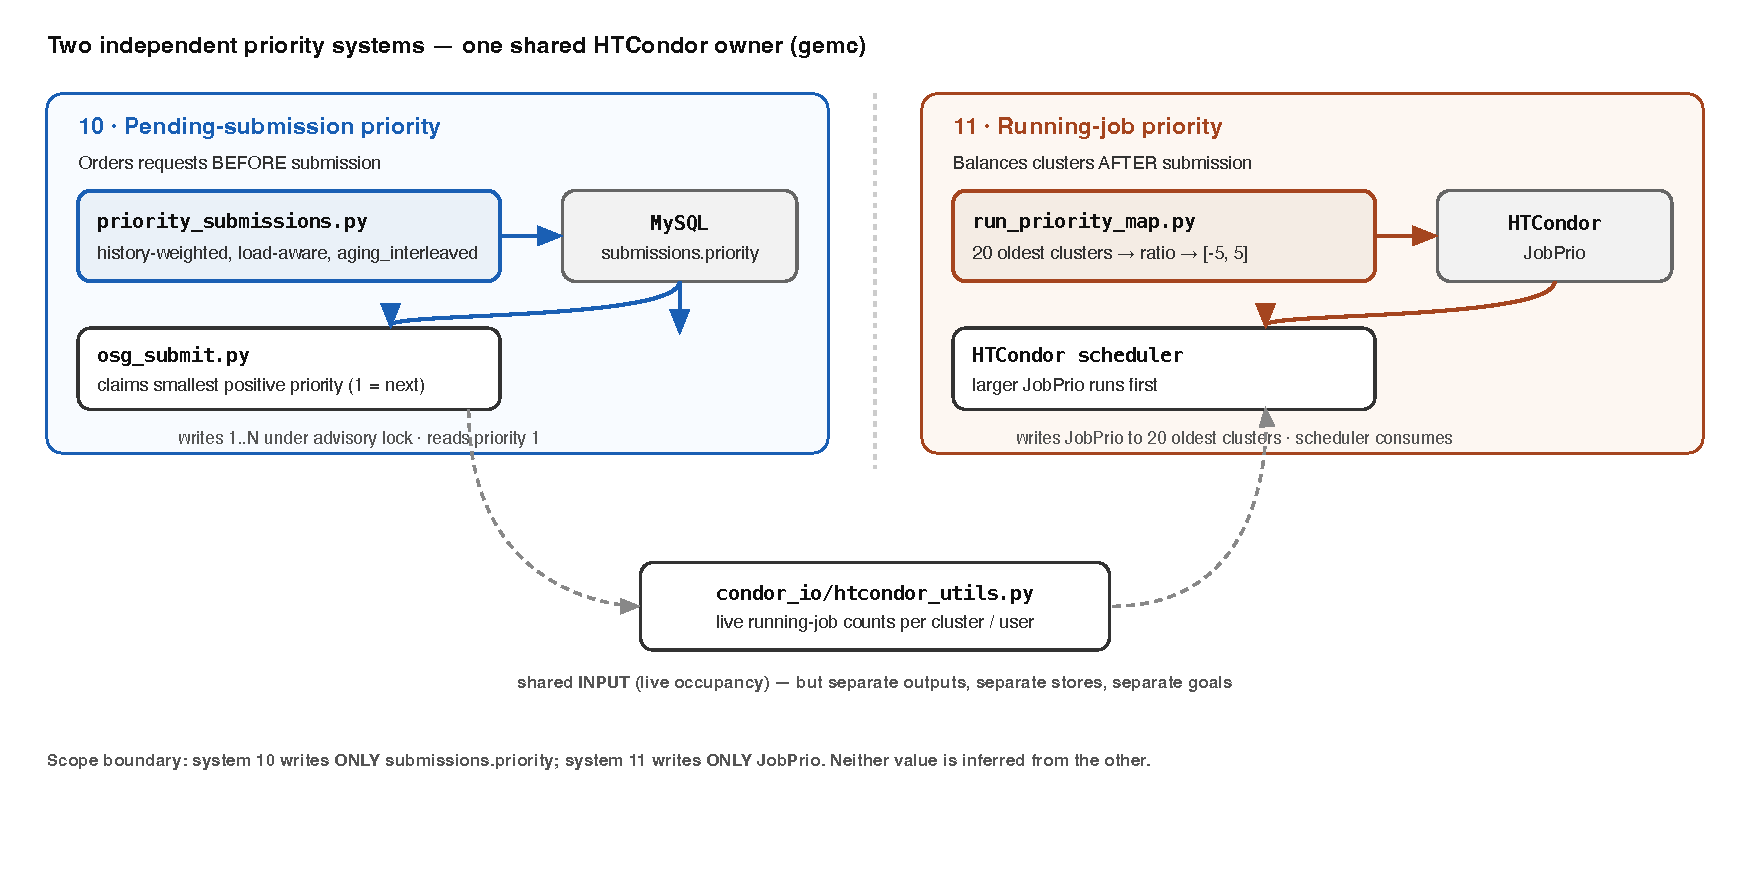
\includegraphics[width=\textwidth]{figures/fig4_two_priorities}
  \caption{The two priority systems share live-occupancy input via \texttt{htcondor\_utils.py} but are
  otherwise strictly separated --- the single most misunderstood aspect of the portal. System~10 writes only
  \texttt{submissions.priority}; system~11 writes only \texttt{JobPrio}; neither value is inferred from the
  other.}
  \label{fig:priorities}
\end{figure}


\section{HTCondor Integration Layer (\texttt{condor\_\allowbreak{}io/\allowbreak{}htcondor\_\allowbreak{}utils.\allowbreak{}py})}\label{ch:12}

\subsection{Schedd querying and batch grouping}

\texttt{htcondor\_\allowbreak{}utils.\allowbreak{}py} is the shared query layer for both priority systems and the monitor. It queries the schedd and groups jobs by \texttt{ClusterId} into per-batch records.

\subsection{Job-status taxonomy and count derivation}

For each batch it derives counts by state --- \texttt{RUN}, \texttt{IDLE}, \texttt{HOLD}, \texttt{OTHER} --- and infers \texttt{DONE} from \texttt{TotalSubmitProcs} minus the jobs still present. These counts feed capacity checks, balancing, and the monitor.

\subsection{Submit-time and priority extraction}

It extracts each batch's submit time (for oldest-cluster selection) and current \texttt{JobPrio}, flagging a batch whose jobs hold mixed priorities so the balancer can treat it as unset.

\subsection{Capacity check}

\texttt{is\_\allowbreak{}under\_\allowbreak{}job\_\allowbreak{}limit()} implements the engine's back-pressure test (running + idle vs. the configured maximum, Chapter 7.2).

\subsection{Behavioral caveats}

The schedd query sees only the live queue, not completed history; \texttt{DONE} is inferred, not read from history. Monitoring accounts for this by snapshotting (Chapter 13).

\section{Monitoring, Display, and Completion}\label{ch:13}

\subsection{Building the submissions view}

\texttt{condor\_\allowbreak{}io/\allowbreak{}list\_\allowbreak{}owner\_\allowbreak{}submission.\allowbreak{}py} builds the portal's submissions table by joining live HTCondor batch counts (total/done/running/idle/held) to the newest matching MySQL row where \texttt{pool\_\allowbreak{}node =\allowbreak{} ClusterId}.

\subsection{Extra rows and de-duplication}

It adds MySQL rows that have not reached HTCondor --- \texttt{Not Submitted} requests and terminal pre-submission failures --- and de-duplicates so each submission appears once.

\subsection{The priority-display substitution}

For a matched submission the script reads the Condor \texttt{JobPrio} but then \textbf{replaces the displayed priority with the MySQL \texttt{submissions.\allowbreak{}priority}.} Consequently the portal table shows the portal-queue position, not the runtime \texttt{JobPrio}; inspect live \texttt{JobPrio} with \texttt{run\_\allowbreak{}priority\_\allowbreak{}map.\allowbreak{}py -\allowbreak{}p}.

\subsection{Snapshotting and pruning}

\texttt{-\allowbreak{}-\allowbreak{}store-\allowbreak{}db} writes the joined view as a JSON snapshot to \texttt{owner\_\allowbreak{}submission\_\allowbreak{}snapshots}, keeping only the newest N (\texttt{prune\_\allowbreak{}owner\_\allowbreak{}submission\_\allowbreak{}snapshots}). \texttt{-\allowbreak{}-\allowbreak{}from-\allowbreak{}db} reads the latest snapshot, decoupling the display from a live schedd query.

\subsection{Progress history}

Reading a window of snapshots yields per-submission progress over time (done-count deltas against the previous snapshot), the basis for the progress column and the estimated-time-remaining figure.

\subsection{Completion detection}

\texttt{db\_\allowbreak{}io/\allowbreak{}mark\_\allowbreak{}completed\_\allowbreak{}submissions.\allowbreak{}py} marks a submission \texttt{Completed} when its cluster has disappeared from the snapshots --- the absence-from-snapshot heuristic --- because the schedd does not retain completed clusters. It defaults to a dry run; writing requires an explicit flag.

\subsection{Front-end rendering}

\texttt{main.\allowbreak{}js} renders the snapshot JSON into the submissions and fair-share tables (\texttt{osgLogtoTable}, \texttt{fairshareToTable}) and computes the estimated time remaining from progress deltas and queue depth.

\subsection{External monitoring links}

The portal links to daily digest emails and the OSG dashboards for pool-level views beyond the portal's own tables.

\subsection{Long-term statistics}

\texttt{stats/\allowbreak{}nsubmission.\allowbreak{}py} and \texttt{stats/\allowbreak{}top\_\allowbreak{}users.\allowbreak{}py} produce long-term submission counts and per-user totals for reporting and capacity planning.

\section{Operations and Deployment}\label{ch:14}

\subsection{Submit-node layout and repository update}

The submit node hosts the repository, the \texttt{\textasciitilde{}/\allowbreak{}venv/\allowbreak{}pymysql} Python environment, and the \texttt{\textasciitilde{}/\allowbreak{}osgOutput/\allowbreak{}} staging tree. \texttt{update\_\allowbreak{}simgrid.\allowbreak{}sh} \textbf{only pulls repository updates} --- it calculates neither priority value, a deliberate separation so a deployment never perturbs the queues.

\subsection{Cron schedule inventory}

Production cron drives the system: the submission engine (\texttt{osg\_\allowbreak{}submit.\allowbreak{}py}), the pending-priority calculation (\texttt{priority\_\allowbreak{}submissions.\allowbreak{}py -\allowbreak{}-\allowbreak{}write-\allowbreak{}to-\allowbreak{}db}), the runtime \texttt{JobPrio} calculation (\texttt{run\_\allowbreak{}priority\_\allowbreak{}map.\allowbreak{}py -\allowbreak{}p -\allowbreak{}a -\allowbreak{}m 20}, every 10 minutes), snapshotting (\texttt{list\_\allowbreak{}owner\_\allowbreak{}submission.\allowbreak{}py -\allowbreak{}-\allowbreak{}store-\allowbreak{}db}), and completion detection (\texttt{mark\_\allowbreak{}completed\_\allowbreak{}submissions.\allowbreak{}py}). The complete inventory is in Appendix G.

\subsection{Locking and single-writer guarantees}

\texttt{run\_\allowbreak{}with\_\allowbreak{}lock\_\allowbreak{}and\_\allowbreak{}log.\allowbreak{}zsh} wraps each cron job so only one instance runs at a time and its output is logged; the MySQL advisory lock (Chapter 5.6) serializes the queue writers. Together they give single-writer guarantees across independent cron jobs.

\subsection{Credentials and secrets}

MySQL credentials live in a connection file (\texttt{msql\_\allowbreak{}conn.\allowbreak{}txt}) read by the \texttt{Database} wrapper; OSDF access uses short-lived OAuth bearer tokens minted by the CredMon. No long-lived grid secret is stored on a worker node.

\subsection{Capacity limits and back-pressure tuning}

The engine's \texttt{-\allowbreak{}-\allowbreak{}max-\allowbreak{}submitted-\allowbreak{}jobs} (default 80,000) bounds the running + idle footprint; production and devel use different maxima. Raising it increases throughput at the cost of a longer local queue.

\subsection{Logging and diagnostics}

Every submission has a per-submission upload log (web tier) and a staging directory with the generated scripts and HTCondor logs; the generated scripts are also stored in the database. Failed submissions leave their staging artifacts for inspection.

\subsection{Runbook}

Common failure modes and recovery: a stuck \texttt{Processing} row (restored on the next engine run via the \texttt{finally} path); a type-2 request failing LUND enumeration (\texttt{Failed to Read Directory} --- check the \texttt{/\allowbreak{}volatile/\allowbreak{}clas12/\allowbreak{}} path); held jobs after 5 retries (inspect the exit code against Appendix E); and back-pressure (normal --- the pool is full). The runbook is expanded in Appendix G.

\section{Testing and Reproducibility}\label{ch:15}

\subsection{Test mode}

\texttt{-\allowbreak{}-\allowbreak{}test} decouples the engine from HTCondor and Pelican: it skips the capacity check, mocks LUND enumeration, performs no MySQL status change, and does not submit. With \texttt{-\allowbreak{}-\allowbreak{}print-\allowbreak{}nodescript} / \texttt{-\allowbreak{}-\allowbreak{}print-\allowbreak{}condor-\allowbreak{}card} it is the standard way to inspect what \textit{would} run for any submission.

\subsection{Unit tests}

\texttt{tests/\allowbreak{}} covers the load-bearing logic: \texttt{test\_\allowbreak{}priority\_\allowbreak{}submissions} (the scoring, ordering, and burst behavior), \texttt{test\_\allowbreak{}lund\_\allowbreak{}helper} (LUND enumeration and the \texttt{lund\_\allowbreak{}files} format), and \texttt{test\_\allowbreak{}mark\_\allowbreak{}completed\_\allowbreak{}submissions} (the absence-from-snapshot heuristic and dry-run default).

\subsection{Reference submissions}

The \texttt{CLAS12TEST} database carries reference submissions 783--787 spanning the pipeline: full workflow (783), GEMC-only with and without background merging (784, 785), and LUND input with and without merging (786, 787). Regenerating their nodescripts and comparing against the stored \texttt{runscript\_\allowbreak{}text} is the standard script-parity check.

\subsection{Container-based verification}

Changes are validated by mounting a work directory into \texttt{jeffersonlab/\allowbreak{}clas12software:\allowbreak{}production} (or \texttt{:\allowbreak{}devel}), copying in \texttt{nodescript.\allowbreak{}sh} and \texttt{functions.\allowbreak{}sh}, and confirming the generator/GEMC/reconstruction command lines are identical to the last known-good submission's stored scripts.

\subsection{Reproducibility guarantees}

The self-documenting nodescript (Chapter 9.1) is the reproducibility guarantee: because every step is an explicit, echoed \texttt{cmd=\allowbreak{}(.\allowbreak{}.\allowbreak{}.\allowbreak{})} array with pinned software versions, a user can copy any step out of a job's log and re-run it verbatim, and the stored \texttt{runscript\_\allowbreak{}text} records exactly what ran.

\section{Security and Trust Model}\label{ch:16}

\subsection{Authentication boundaries}

Two identity domains meet in the portal. Users authenticate to the portal via the web server
(\texttt{REMOTE\_\allowbreak{}USER}), which sets attribution and the output namespace. Jobs authenticate to
OSDF via a single OAuth service (\texttt{jlab\_\allowbreak{}clas12}) under the shared owner \texttt{gemc}. The
portal is the bridge and the only place per-user identity is enforced.

\subsection{Input validation and injection surfaces}

The main injection surfaces are the PHP $\rightarrow$ shell boundary (the \texttt{exec} of the uploader) and
the scard parser. The portal escapes fields and quotes shell arguments (\texttt{escapeshellarg}), restricts the
string identifier to a safe character class at input, and the scard parser treats unknown keys as inert data
(\texttt{\_\allowbreak{}extra}) rather than executing them.

\subsection{Path and namespace isolation}

Type-2 inputs are constrained to \texttt{/\allowbreak{}volatile/\allowbreak{}clas12/\allowbreak{}} (enforced
before any file operation), and outputs are written to a per-user OSDF namespace
(\texttt{.\allowbreak{}.\allowbreak{}.\allowbreak{}/\allowbreak{}osg/\allowbreak{}<user>/\allowbreak{}%
<sub\_\allowbreak{}id>/\allowbreak{}}), so one user's request cannot read or overwrite another's area.

\subsection{Token lifetime and least privilege}

The CredMon mints short-lived bearer tokens per job; no long-lived credential is transferred to a worker node,
so a compromised slot exposes at most a short-lived, narrowly-scoped token.

\section{Discussion, Limitations, and Future Work}\label{ch:17}

\subsection{Known limitations}

Fair sharing is implemented on top of a single shared HTCondor owner, so it is only as good as the portal's own bookkeeping; queue-time estimates use a static per-job constant rather than measured throughput; and completion is a heuristic (absence from snapshots) rather than a definitive per-job signal.

\subsection{Scalability considerations}

The pending-queue recalculation and the snapshot joins scale with the number of active submissions and live clusters; the advisory lock serializes queue writes, which is correct but a single writer. At much larger scale the snapshot cadence and the schedd-query cost would be the first things to profile.

\subsection{Possible improvements}

Candidate improvements include per-user (rather than per-cluster) runtime balancing if OSG accounting ever distinguishes portal users, throughput-based rather than static queue estimates, and unifying the two priority telemetries into one view while preserving their strict separation of concerns.

\subsection{Lessons learned}

The design's most durable decision is the strict separation of the two priority systems: a pending queue that decides \textit{what to submit} and a runtime map that decides \textit{what to run}, each with a single writer and a single store. Keeping them apart --- in the code, the docs, and this note --- is what keeps the system's behavior predictable under a shared grid identity.

\section{Conclusion}\label{ch:18}

simGrid turns a browser form into a fair-shared, reproducible CLAS12 Monte-Carlo workflow on opportunistic OSG
resources. A scard captures the request; a MySQL-backed state machine and a locked contiguous queue order it; a
submission engine generates a self-documenting HTCondor cluster and worker-node pipeline; and two deliberately
separate priority systems keep the shared allocation fair before and after submission. The combination of
self-service submission, pinned-software reproducibility, eviction-tolerant retry, and explicit fair sharing
has made large-scale CLAS12 simulation a routine, self-service operation rather than an expert task.


\appendix
\section{Scard field reference}

Complete list of scard keys parsed by \texttt{SConfiguration}, their meaning, defaults, and consumers. Fields: \texttt{project}, \texttt{type} (1/2, inferred if absent), \texttt{connection}, \texttt{version}, \texttt{username}, \texttt{configuration}, \texttt{generator} (name $\rightarrow$ type-1, path/URL $\rightarrow$ type-2), \texttt{genOptions}, \texttt{nevents}, \texttt{njobs}/\texttt{jobs}, \texttt{client\_\allowbreak{}ip}, \texttt{fields} (\texttt{tor<T>\_\allowbreak{}sol<S>}), \texttt{torus}, \texttt{solenoid}, \texttt{bkmerging}, \texttt{softwarev} (\texttt{gemc/\allowbreak{}\ldots{} coatjava/\allowbreak{}\ldots{} mcgen/\allowbreak{}\ldots{}}), \texttt{dstOUT}, \texttt{zposition}, \texttt{raster}, \texttt{beam}, \texttt{vertex\_\allowbreak{}choice}, \texttt{string\_\allowbreak{}id}/\texttt{user\_\allowbreak{}string}, \texttt{output\_\allowbreak{}type} (0 DST / 1 GEMC-only), \texttt{submission}, \texttt{runs}, \texttt{run\_\allowbreak{}list}, \texttt{gemcv}/\texttt{coatjavav}/\texttt{mcgenv} (derived), \texttt{genExecutable}. Unknown keys are retained in \texttt{\_\allowbreak{}extra}. \textit{(To be rendered as a full table in the Pages document.)}

\section{Submission-database schema (DDL)}

DDL for \texttt{submissions} (columns \texttt{user\_\allowbreak{}submission\_\allowbreak{}id}, \texttt{user}, \texttt{client\_\allowbreak{}time}, \texttt{server\_\allowbreak{}time}, \texttt{pool\_\allowbreak{}node}, \texttt{scard}, \texttt{run\_\allowbreak{}status}, \texttt{priority}, \texttt{runscript\_\allowbreak{}text}, \texttt{clas12\_\allowbreak{}condor\_\allowbreak{}text}), \texttt{users}, and \texttt{owner\_\allowbreak{}submission\_\allowbreak{}snapshots} (\texttt{snapshot\_\allowbreak{}id}, \texttt{update\_\allowbreak{}time}, \texttt{database\_\allowbreak{}name}, \texttt{owner}, \texttt{payload\_\allowbreak{}json}). \textit{(Extract the authoritative DDL from the production schema before release.)}

\section{Annotated HTCondor submit-file example}

A full generated \texttt{clas12.\allowbreak{}condor} (type-1 and type-2), annotated section by section against Chapter 8. Generate with \texttt{osg\_\allowbreak{}submit.\allowbreak{}py -\allowbreak{}b <ID> -\allowbreak{}-\allowbreak{}test -\allowbreak{}-\allowbreak{}print-\allowbreak{}condor-\allowbreak{}card}.

\section{Annotated \texttt{nodescript.\allowbreak{}sh} example}

Full generated nodescripts for a full-DST type-1 job and a GEMC-only type-2 job, annotated against Chapter 9. Generate with \texttt{osg\_\allowbreak{}submit.\allowbreak{}py -\allowbreak{}b <ID> -\allowbreak{}-\allowbreak{}test -\allowbreak{}-\allowbreak{}print-\allowbreak{}nodescript [-\allowbreak{}-\allowbreak{}devel]}.

\section{Exit-code catalogue and \texttt{periodic\_\allowbreak{}release} mapping}

The nodescript exit codes and which are treated as transient by the Condor card (202, 204--208, 210--213 $\rightarrow$ retried up to 5 times after a 1-hour hold; all others $\rightarrow$ held for inspection).

\section{Priority-algorithm parameter reference and worked example}

Reference for \texttt{-\allowbreak{}-\allowbreak{}priority-\allowbreak{}algorithm}, \texttt{-\allowbreak{}-\allowbreak{}half-\allowbreak{}life-\allowbreak{}days}, \texttt{-\allowbreak{}-\allowbreak{}history-\allowbreak{}half-\allowbreak{}life-\allowbreak{}days}, \texttt{-\allowbreak{}-\allowbreak{}queue-\allowbreak{}penalty-\allowbreak{}exponent}, \texttt{-\allowbreak{}-\allowbreak{}burst-\allowbreak{}per-\allowbreak{}user}, \texttt{-\allowbreak{}-\allowbreak{}no-\allowbreak{}queue-\allowbreak{}penalty}, \texttt{-\allowbreak{}d}, \texttt{-\allowbreak{}-\allowbreak{}condor-\allowbreak{}owner}, with a worked numerical example of \texttt{aging\_\allowbreak{}interleaved} ordering two users' pending rows given their running counts and histories.

\section{CLI reference}

All scripts and flags: \texttt{osg\_\allowbreak{}submit.\allowbreak{}py}, \texttt{db\_\allowbreak{}io/\allowbreak{}upload\_\allowbreak{}submission.\allowbreak{}py}, \texttt{db\_\allowbreak{}io/\allowbreak{}priority\_\allowbreak{}submissions.\allowbreak{}py}, \texttt{condor\_\allowbreak{}io/\allowbreak{}run\_\allowbreak{}priority\_\allowbreak{}map.\allowbreak{}py}, \texttt{condor\_\allowbreak{}io/\allowbreak{}list\_\allowbreak{}owner\_\allowbreak{}submission.\allowbreak{}py}, \texttt{db\_\allowbreak{}io/\allowbreak{}mark\_\allowbreak{}completed\_\allowbreak{}submissions.\allowbreak{}py}, \texttt{db\_\allowbreak{}io/\allowbreak{}database.\allowbreak{}py -\allowbreak{}q}, and the \texttt{stats/\allowbreak{}} scripts, plus the production cron inventory.

\section{Glossary}

CLAS12, GEMC, OSG, HTCondor, glidein/pilot, CVMFS, Singularity/Apptainer, Pelican, OSDF, CredMon, scard, gcard, cluster, subjob, \texttt{ClusterId}, \texttt{JobPrio}, \texttt{pool\_\allowbreak{}node}, type-1, type-2, DST, LUND, RCDB.

\section{File/module map}

Repository layout mapped to responsibility: \texttt{osg\_\allowbreak{}submit.\allowbreak{}py}, \texttt{SConfiguration.\allowbreak{}py}, \texttt{statuses.\allowbreak{}py}, \texttt{db\_\allowbreak{}io/\allowbreak{}} (database, upload, priority, completion), \texttt{condor\_\allowbreak{}io/\allowbreak{}} (htcondor utils, priority map, listing), \texttt{generators/\allowbreak{}condor/\allowbreak{}} (nine card sections), \texttt{generators/\allowbreak{}bash/\allowbreak{}} (nodescript sections, run selection), \texttt{web\_\allowbreak{}portal/\allowbreak{}} (PHP pages, \texttt{main.\allowbreak{}js}), \texttt{stats/\allowbreak{}}, and \texttt{tests/\allowbreak{}}.




% ============================ REFERENCES =====================================

% =============================================================================
%  CLAS12 Technical Note --- references
%
%  The recurring foundational CLAS12-note references reused across the beam-
%  background notes (authoring guide, section 7). Cite with \cite{key}; keep the
%  entries you use and add note-specific references below.
% =============================================================================

\begin{thebibliography}{9}

\bibitem{note:moller}
  R.~De Vita and M.~Ungaro,
  {\it CLAS12-note 2016-006: Moller shield --- GEMC-optimized layout vs.\ the
  engineering design.}

\bibitem{note:beamline}
  R.~De Vita {\it et al.},
  {\it CLAS12-note 2017-012: Corrections to the CLAS12 vacuum beamline.}

\bibitem{note:target}
  M.~Ungaro,
  {\it CLAS12-note 2017-013: Corrections to the CLAS12 target design.}

\bibitem{note:embg}
  R.~De Vita {\it et al.},
  {\it CLAS12-note 2017-016: Electromagnetic background rates in CLAS12.}

\bibitem{note:cad}
  R.~De Vita and M.~Ungaro,
  {\it CLAS12-note 2017-017: Importing the CLAS12 CAD models of the target and
  beamline.}

\bibitem{note:ftof}
  D.~Carman,
  {\it FTOF-note 2014-06: Forward Time-of-Flight PMT currents.}

\bibitem{gemc:epj}
  M.~Ungaro,
  {\it GEMC: A database-driven simulation program,}
  EPJ Web Conf.\ {\bf 295} (2024).

\bibitem{gemc:nim}
  M.~Ungaro {\it et al.},
  {\it The CLAS12 Geant4 simulation,}
  Nucl.\ Instrum.\ Meth.\ A {\bf 959} (2020) 163422.

\end{thebibliography}



% ============================ ALL DONE =====================================
\end{document}


